%%%%%%%%%%%%%%%%%%%%%%%%%%%%%%%%%%%%%%%%%%%%%%%%%
%
%     Chapter 5
%
%%%%%%%%%%%%%%%%%%%%%%%%%%%%%%%%%%%%%%%%%%%%%%%%

\chapter{Implementation}
\label{five}

In this Chapter, we describe our realization of Parabix technology inside LLVM facility. LLVM is a well-structured open source compiler tool chain which is under rapid development. So during our implementation, we tried our best to follow its design principle while keeping our code modularized and isolated to be able to easily integrate with new versions of LLVM\@. Our goal of code design is to:
\begin{enumerate}
  \item Use general strategies across different types and operations to reduce repeated logic.
  \item Minimize code injection in the existing source and put Parabix logic in the separate module.
  \item Check correctness of every operation we implement. Since most of the test code follow the same pattern, they should be generated automatically to reduce repeated human work.
\end{enumerate}

Most of our code sit in LLVM Target-Independent Code Generator\cite{llvm_code_gen}. From Chapter~\ref{four}, we know that the current type legalization process of LLVM has big performance penalty for small element vectors. So our approach marks $i1$, $i2$ and $i4$ vector legal type first, and then handle them in the operation legalization phase. For convenience, we name this set of vector types \textit{Parabix Vector}.

We walk through the following steps to mark a type legal on a certain target:
\begin{itemize}
  \item \textbf{Add new register class in target description file.} LLVM uses TableGen (.td files) to describe target information which allows the use of domain-specific abstractions to reduce repetition \cite{llvm_code_gen}. Registers are grouped into register classes which further tie to a set of types. We introduced GR32X for 32-bit general register like EAX EBX for $v32i1$, GR64X for 64-bit general register like RAX RBX for $v64i1$, VR128PX for 128-bit vector register like XMM0 to XMM15 for $v128i1$, $v64i2$, $v32i4$  Types within the same register class can be bitcasted from one to the other, since they can actually reside in the same register.

  \item \textbf{Set calling convention.} They are two kinds of calling convention to set: return value and argument calling convention. For example, we instruct LLVM to assign $v64i2$ type return value to XMM0 to XMM3 registers, assign $v64i2$ argument type to XMM0 to XMM3 registers if SSE2 is available or to 16-byte stack slots otherwise.
\end{itemize}

Now the type legalization phase recognizes our $i1$, $i2$, $i4$ vectors as legal and passes them onto the operation legalization phase. We have two major methods to handle $i2^k$ vectors: \textit{Custom Lowering} and \textit{DAG Combining}.

\begin{figure}[ht!]
\centering
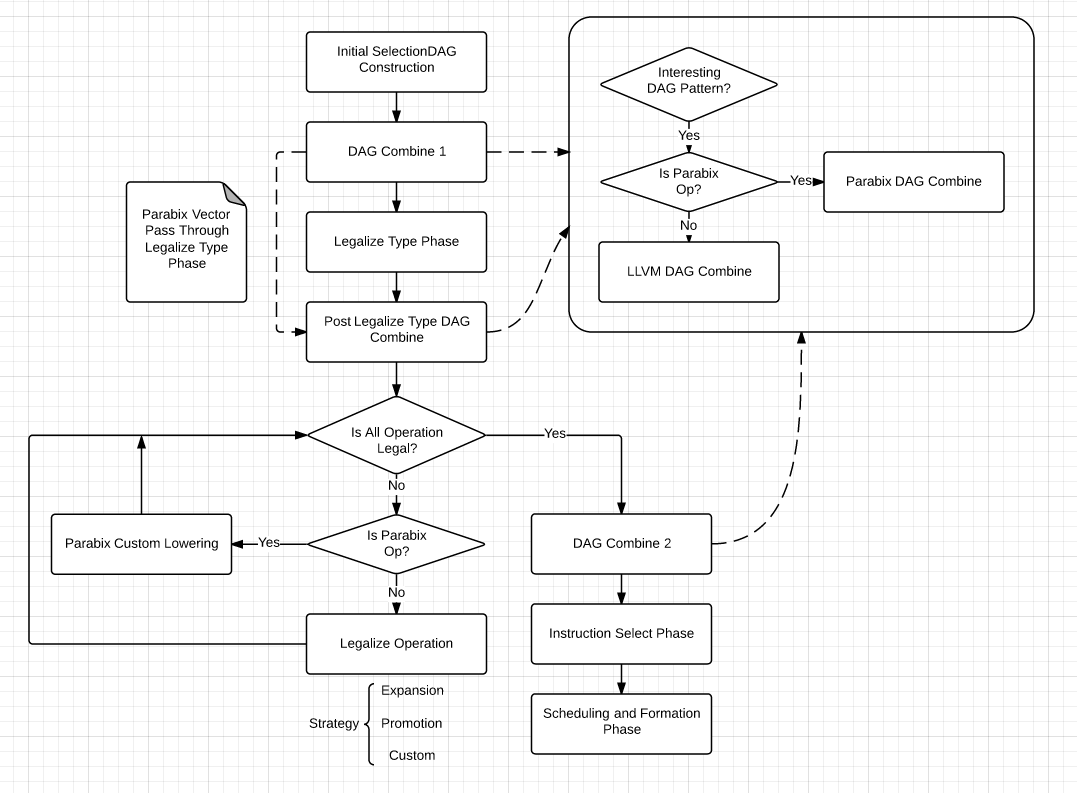
\includegraphics[width=140mm]{draw/system.png}
\caption[System overview: modified instruction selection process]{Overview of the modified instruction selection process. Logic for Parabix vectors are hooked into two places: the operation legalization phase and DAG Combine Phases.}
\label{figure:system}
\end{figure}

Figure~\ref{figure:system} gives an overview of our implementation. LLVM constructs a SelectionDAG with the input IR source code and then puts it through DAG Combine 1 for cleaning up and optimization. The optimized DAG is fed into the type legalization phase. We mark the Parabix Vectors type-legal so that they could pass through this phase without being changed. There is another DAG combining phase after the type legalization. Then, the result DAG is fed into the operation legalization phase which is done by iteration. Custom Lowering for Parabix resides in this phase. In each iteration, the legalizer checks every DAG node for its legality. If the node is illegal and performs operation on some Parabix vector, the Parabix Custom Lowering code will be called to legalize this node; otherwise the default LLVM logic will handle this illegal node. The iteration terminates when every DAG node is legal. By iteration, the legalizer could introduce new illegal nodes into the graph.

After the operation legalization phase, there is another DAG combining to clean up the messy output. The last two steps for machine code generation remain the same. There are Parabix DAG Combine logic in all the three DAG combining phases. Each DAG combining phase maintains a work list. It traverses the DAG graph for specific operations. If the operation works with Parabix vectors and it fits certain pattern, the Parabix DAG Combine logic will replace the node with a new node or a new sub-tree of nodes. Part(or all) of the new nodes can be appended to the work list so that the legalizer knows to combine it further later. There is not built-in iteration for DAG combining, but the iteration can be emulated by keeping appending the processed nodes to the work list if necessary.

In the following sections, we discuss some custom lowering strategies and how they are organized to fit our design goal; then we give some examples of the Parabix DAG Combiner which are usually special cases for a certain operation; finally we show how we use templates to generate code and test cases for the sake of DRY (don't repeat yourself).

\section{Standard Method For Custom Lowering}
\subsection{Custom Lowering Strategies}
After the type legalization phase, one shall not generate illegal types again. This means all the phases after type legalization are target-specific. But in practice, almost all the targets support $i8$, $i32$ and $i64$, so there are still general strategies we can apply across targets. For different types like $v32i1$ and $v128i1$, general strategies also exist to lower both of them. We define three legalize actions as the following:
\begin{enumerate}
    \item Bitcast to full register and replace the operation code. This is useful for all $i1$ vectors, we need to specify the new operation code when defining the action, e.g.\ XOR for ADD on $v32i1$.
    \item In-place promotion. Automatically apply $i2X$ vector operations on $iX$ vector following the Inductive Doubling Principle.
    \item Custom. Same concept with LLVM Custom Lowering, manually replace an illegal DAG node with a sequence of new DAG nodes. They can be illegal nodes, but they cannot introduce illegal types. All $i2$ vectors are lowered here, also the 1-add version of the $v32i4$ addition.
\end{enumerate}

\subsection{DAG Combiner}
\label{sec:long_shift}
DAG Combiner is the supplement to custom lowering facility. It often focuses on special cases e.g.\ one operation and a subset of possible operands. We give a few examples of Parabix DAG Combiner here.

\begin{figure}[htbp!]
\centering
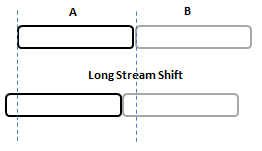
\includegraphics[scale=0.8]{draw/long_shift.png}
\caption{Long stream shifting}
\label{fig:long_shift}
\end{figure}

\begin{figure}[htbp!]
\centering
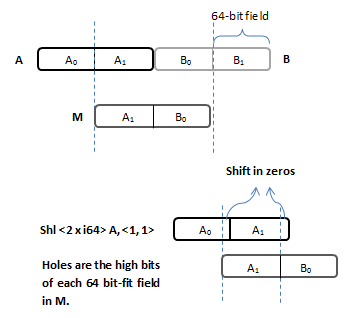
\includegraphics[scale=0.9]{draw/long_shift_good.png}
\caption{A better algorithm for long stream shift.}
\label{fig:long_shift_good}
\end{figure}

We first show a peephole optimization that greatly improves the performance of long stream shifting. Long stream shifting shifts left one whole SIMD register with potential shift-in bits from the other SIMD register. Refer to Figure~\ref{fig:long_shift}, we want to shift left {\tt A} by $n$ bits and shift-in the highest $n$ bits from B. To be simple, we assume $n = 1$ and the SIMD register is 128-bit wide. The most straight-forward implementation is listed below:
  \[ \text{\tt A1 = shl i128 A, 1} \]
  \[ \text{\tt B1 = lshr i128 B, 127} \]
  \[ \text{\tt R = or i128 A1, B1} \]
This algorithm is called double shift. It describes clearly what we want to implement so it is the preferred IR code in the library. Since shift on $i128$ is not natively supported, double shifts of $v2i64$ and one shufflevector are needed to implement the $i128$ shift. Thus, we need 4 $v2i64$ shifts, 2 shufflevectors and 3 logic or operations. The $v2i64$ shifts take most of the run time.

\begin{figure}[htbp!]
\centering
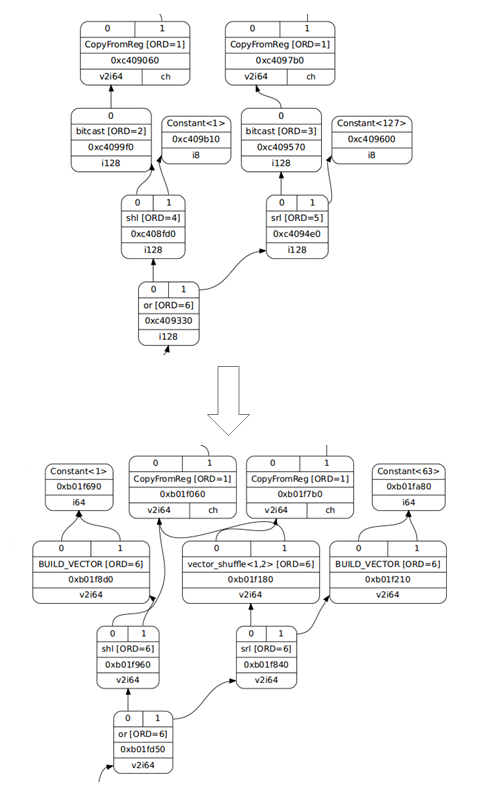
\includegraphics[scale=0.8]{draw/long_shift_nodes.png}
\caption[The DAG combiner for long stream shift.]{The DAG combiner for long stream shift. When the above pattern is recognized, it gets replaced with the better implementation below.}
\label{fig:long_shift_nodes}
\end{figure}

A better algorithm that uses 2 $v2i64$ shifts, 1 shufflevector and 1 logic or is implemented. Refer to Figure~\ref{fig:long_shift_good}, the algorithm is listed below:
  \[ \text{\tt M = shufflevector <2 x i64> A, B, <2 x i32> <i32 1, i32 2>} \]
  \[ \text{\tt D = shl <2 x i64> A, <2 x i64> <i32 1, i32 1>} \]
  \[ \text{\tt E = lshr <2 x i64> M, <2 x i64> <i32 63, i32 63>} \]
  \[ \text{\tt R = or <2 x i64> D, E} \]

{\tt M} is the key to this algorithm. When we shift left {\tt A} as $v2i64$, we create holes (1-bit shift-in zeros) in the lower end of each field. The correct fill-in data for these holes are just the highest bit in each field of {\tt M}. So we shift right {\tt M} as $v2i64$ to align the bits into correct positions and use logic or operation to fill the holes. This algorithm can be generalized to long stream shift with arbitrary amount.

Once the back end recognizes the double-shift code, it re-implements with the better algorithm. The DAG combining process is described in Figure~\ref{fig:long_shift_nodes}.

The next example is shufflevector for {\tt hsimd<16>::packh}. With the similar code described in Chapter~\ref{three}, LLVM 3.4 does not generate the best assembly code. It generates a sequence of $pextrw$ and $pinsrw$. Even the newst LLVM truck generates 27 lines of assembly. We create the following DAG Combiner and get the 5 lines of equivalent assembly code in Program~\ref{prog:packh_16_asm}.
\begin{itemize}
    \item \textbf{Pattern}: shufflevector on $v16i8$ with mask = 1, 3, 5, \ldots, 31.
    \item \textbf{Combine Result}: one PACKUS node, which unsigned saturates two $v8i16$ into $v8i8$ vectors and concatenates them into one $v16i8$.
\end{itemize}

\begin{program}[htbp!]
\begin{verbatim}
    psrlw   $8, %xmm0
    psrlw   $8, %xmm1
    packuswb    %xmm0, %xmm1
    movdqa  %xmm1, %xmm0
    retq
\end{verbatim}
\caption{The optimized assembly code for {\tt hsimd<16>::packh}}
\label{prog:packh_16_asm}
\end{program}

\FloatBarrier
The efficient implementation of {\tt packh} on vectors of small elements are possible with the PEXT instruction introduced by the Intel Haswell BMI2. PEXT is a useful instruction for bit manipulation on $i32$ and $i64$. Given the $i8$ variable A = $(\text{abcdefgh})_2$, Mask = $(10101010)_2$, PEXT(A, Mask) returns R = $(\text{aceg})_2$. PEXT extracts bits from A at the corresponding bit locations specified by the mask. With this in mind, we can implement \verb|hsimd<2>::packh| as Program~\ref{program:packh_2} (in pseudo IR for readability).

\begin{program}[htbp!]
\begin{verbatim}
    define <2 x i64> @packh_2(<2 x i64> A, <2 x i64> B) {
    entry:
      ; extract lower 64 bits (A0) and higher 64 bits (A1)
      A0 = extractelement <2 x i64> A, i32 0
      A1 = extractelement <2 x i64> A, i32 1

      Mask = 0xAAAAAAAAAAAAAAAA ; 1010...1010 in binary
      P0 = PEXT(A0, Mask) | (PEXT(A1, Mask) << 32)

      ; same for B
      B0 = extractelement <2 x i64> B, i32 0
      B1 = extractelement <2 x i64> B, i32 1
      P1 = PEXT(B0, Mask) | (PEXT(B1, Mask) << 32)

      ret <2 x i64> <i64 P0, i64 P1>
    }
\end{verbatim}
\caption{Implementation of {\tt hsimd<2>::packh} with PEXT.}
\label{program:packh_2}
\end{program}

According to Program~\ref{program:packh_2}, we create the following DAG Combiner:
\begin{itemize}
    \item \textbf{Pattern}: shufflevector on $v128i1$, $v64i2$ or $v32i4$ with mask = 0, 2, 4, \ldots, $NumElt \times 2-2$ or mask = 1, 3, 5, \ldots, $NumElt \times 2 -1$. $NumElt$ is the number of elements for each type e.g.\ $NumElt=32$ for $v32i4$.
    \item \textbf{Combine Result}: four PEXT nodes combined with OR and SHL.
\end{itemize}

To summarize, this kind of DAG Combiner provides a shortcut for the programmer to do peephole optimization. It can co-exist with a full custom lowering, like the relationship between immediate shifting and arbitrary shifting. Immediate shifting shifts all the vector elements with the same amount, allowing efficient realization for $v32i4$ with $v4i32$ shifts, while we apply In-place Promotion strategy for $v32i4$ arbitrary shifting in the Parabix custom lowering.

DAG Combiner can optimize operations with illegal type in the phase DAG Combine 1. It is not possible in the custom lowering. But we cannot simply put all the Parabix Custom Lowering logic inside the DAG Combiner. First, it is against LLVM design; DAG Combiner is designed for cleaning up, either the initial code or the messy code generated by the legalization passes \cite{llvm_code_gen}. Second, it cannot utilize the legalization iteration; in custom lowering, general strategies may introduce new illegal operations which are hard to avoid since "illegal" is a target-specific concept. The DAG Combiner, on the other hand, 1) Should not generate illegal operations in the phases after the operation legalization phase. 2) Although it can also work in iteration, most of the lowering logic for common operations are not programmed in this module, we would end up with illegal non-Parabix operations.

\section{Templated Implementation}
During our implementation, we encountered much duplicated code, especially in the test cases; Such duplication is against software design principles and is hard to maintain, sometimes even hard to write; a thorough test file for $i2^k$ vector contains more than two thousand lines of code, most of which are in the same pattern. To keep DRY and save programmer time, we introduced Jinja template engine \cite{jinja_engine}. According to \cite{python_templating}, Jinja belongs to the Engines Mixing Logic into Templates, it allows embedding logic or control-flow into template files. We use Jinja because:

\begin{itemize}
    \item We can write all pieces of the content in one file, so it is easier to understand. Where in the Engines using Value Substitution, the driver code usually contains many tiny pieces of content. The reader must read the driver code as well as the template file to understand the output. One template example can be found in Program~\ref{program:jinja}.
    \item Like the standard Model-View-Controller structure in the web design, our driver code needs only provide abstract data (like operation names in IR and the corresponding C++ library calls). How to present these data is not its responsibility. In the other word, we can have significant changes in the template without changing the driver.
    \item Jinja uses python and python is easy and quick to use.
\end{itemize}

\subsection{Code Generation For $i2$ Vector}
In Chapter~\ref{four}, we legalized $i2$ vector operations with boolean functions. In our implementation, with the Quine-McCluskey solver, we got 11 sets of formula which reside in one compact data script. We wrote template files to generate 11 C++ functions for them. This approach has the following benefits:
\begin{itemize}
    \item Collect all the critical formula together so that possible future updates are easy to deploy.
    \item Implementation details only reside in the template file, so we are able to change the code structure easily. For now we create one function for each formula, but it is possible that we plan to create one big switch statement and generate one case for each formula instead. This can be done with only a few lines of change in the template.
\end{itemize}

Example formula of $v64i2$ addition as well as the function template is listed in the Program~\ref{prog:i2_codegen} and Program~\ref{prog:i2_func_template}.

\begin{program}[htbp!]
\begin{verbatim}
    "add_2": r'''
        tmp = simd_xor(arg1, arg2)
        return simd_ifh1(simd_himask(fw),
                         simd_xor(tmp, simd_slli(1, simd_and(arg1, arg2))), tmp)
    '''
\end{verbatim}
\caption[Minimum boolean function for $v64i2$ addition]{Minimum boolean function for $v64i2$ addition.}
\label{prog:i2_codegen}
\end{program}

\begin{program}[htbp!]
\begin{verbatim}
    
    /* Generated function */
    static SDValue GENLower{{ name.op }}(SDValue Op, SelectionDAG &DAG) {
      MVT VT = Op.getSimpleValueType();
      MVT FullVT = getFullRegisterType(VT);
      SDNodeTreeBuilder b(Op, &DAG);

      if (VT == MVT::v64i2) {
        SDValue A1 = b.BITCAST(Op.getOperand(0), FullVT);
        SDValue A2 = b.BITCAST(Op.getOperand(1), FullVT);

    
        {{ line | trim }};
    
      }

      llvm_unreachable("GENLower of {{ name.op }} is misused.");
      return SDValue();
    }

    
\end{verbatim}
\caption[Custom lowering function template for $v64i2$]{Custom lowering function template for $v64i2$. This template file generates one function for each operation.}
\label{prog:i2_func_template}
\end{program}

\subsection{Test Code And IR Library Generation}
We test correctness of our modified LLVM back end by comparing results with the IDISA library. For example we extend LLVM to support $i1$ vectors, but does the extention work? We answer this question by first constructing a IR library of all the functions on $i1$ such as the {\tt add\_1} listed in the top left corner in Figure~\ref{figure:test}. We then write a driver to generate random test data, put them through the IR functions as well as the corresponding IDISA functions, check if the results are the same.

There is one problem in this approach. The driver and IDISA are both written in C++ but the IR library is in low-level representation. How to mix them together? We solve the problem by compiling the IR code into object files. A seperate header file of IR-function signatures is maintained so that the driver code can call IR functions as external functions. The overview of the test system can be found in Figure~\ref{figure:test}. We use templates for both the IR library and the driver, some sample templates can be found in Program~\ref{program:jinja}.


\begin{figure}[hbpt!]
\centering
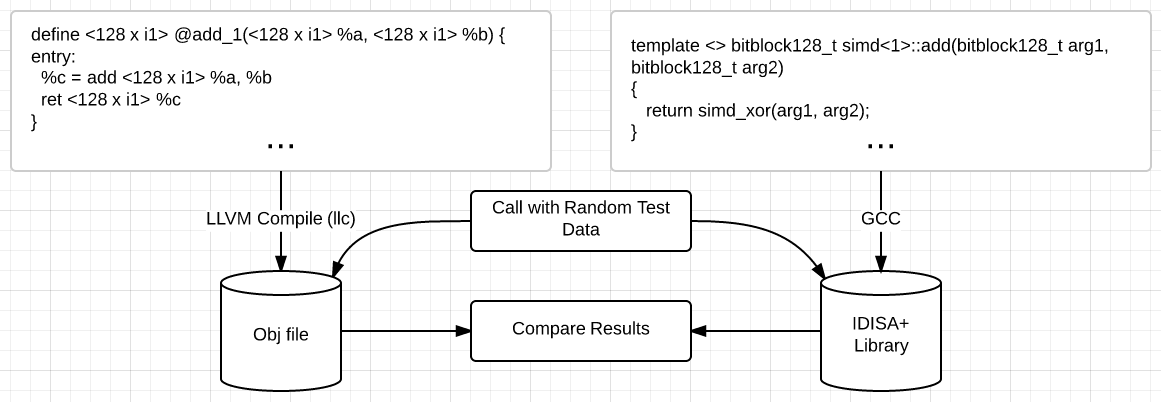
\includegraphics[width=140mm]{draw/test.png}
\caption[Test system overview.]{Test system overview. The pure IR library is first compiled into the native object file and then linked with the driver. The driver call functions from the both side to check correctness.}
\label{figure:test}
\end{figure}

\begin{program}
\begin{verbatim}

define <32 x i4> @{{name.c}}(<32 x i4> %a,
                             <32 x i4> %b)
{
entry:
  %c = {{ name.op }} <32 x i4> %a, %b
  
  %d = sext <32 x i1> %c to <32 x i4>
  ret <32 x i4> %d
  
  ret <32 x i4> %c
  
}

\end{verbatim}
\rule{\textwidth}{1pt}

\begin{multicols}{2}
\begin{verbatim}
define <32 x i4> @add_4(<32 x i4> %a,
                        <32 x i4> %b)
{
entry:
  %c = add <32 x i4> %a, %b
  ret <32 x i4> %c
}
\end{verbatim}
\columnbreak
\begin{verbatim}
define <32 x i4> @eq_4(<32 x i4> %a,
                       <32 x i4> %b)
{
entry:
  %c = icmp eq <32 x i4> %a, %b
  %d = sext <32 x i1> %c to <32 x i4>
  ret <32 x i4> %d
}
\end{verbatim}
\end{multicols}
\caption[Templates for the IR Libray]{Templates for the IR Library. On the top is the template, and two different output are listed below. We use embedded for loop and if statements.}
\label{program:jinja}
\end{program}
